
\documentclass[11pt]{../../classes/ifscarticle}
\usepackage{../../classes/ifscutils}
\usepackage[alf]{abntex2cite} % Citações padrão ABNT
\usepackage[nottoc]{tocbibind}
\renewcommand*{\theusecase}{UC-\thesection.\arabic{usecase}}
\usepackage{lipsum}

\AtBeginDocument{\thispagestyle{empty}}
\begin{document}

% ------------------------------------------------------------%
% Capa
% -------1-----------------------------------------------------%
\begin{center}

    {\large Universidade Estadual Norte Fluminense}\\[0.2cm] %0,2cm é a distância entre o texto dessa linha e o texto da próxima
    {\large Banco de Dados - Prof(a). Sahudy Montenegro }\\[0.2cm] % o comando \\ "manda" o texto ir para próxima linha
    {\large Ciência da Computação}\\[5.2cm]


    % Título
    {\Huge \bfseries Grupo 18 - PEA Pescarte}

    \vspace{.5cm}

    % Subtítulo
    {\LARGE \bfseries Fase Intermediária}

    \vfill
\end{center}
\begin{tabbing}

\end{tabbing}

{\noindent \large \bfseries
Javier Ernesto Lopez Del Real
\\[.5em] Matheus de Souza Pessanha
}


\begin{flushright}
    Data de entrega: 29 de mar\c{c}o de 2021
\end{flushright}

\clearpage
\pagestyle{firstpage}


% ------------------------------------------------------------%
% Adicionando sumário
% ------------------------------------------------------------%
\tableofcontents
\clearpage

% ------------------------------------------------------------%
% Início do documento
% ------------------------------------------------------------%

\section{Introdução}
\label{sec:introducao}

O Projeto de Educação Ambiental(PEA) PESCARTE tem como sua principal finalidade a criação de uma rede social regional integrada por pescadores artesanais e por seus familiares, buscando, por meio de processos educativos, promover, fortalecer e aperfeiçoar a sua organização comunitária e a sua qualificação profissional, bem como o seu envolvimento na construção participativa e na implementação de projetos de geração de trabalho e renda.
\begin{figure}[ht]
    \centering
    
\includegraphics[width=.5\linewidth]{figuras/logoPescarte}
    \caption{Logo do Pescarte}
    \label{fig:logolatex}
\end{figure}

\section{Descrição do problema}

O PEA PESCARTE é divido por quatro núcleos:
\begin{itemize}
    \item Núcleo A
    \item Núcleo B
    \item Núcleo C
    \item Núcleo D
\end{itemize}
Esses Núcleos são compostos por 21(Vinte e uma) linhas
de pesquisa que por sua vez são formadas por
diversos pesquisadores. Um pesquisador possui três tipos:
\begin{itemize}
    \item Pesquisador de Iniciação Científica
    \item Pesquisador de mestrado
    \item Coordenador
\end{itemize}
Cada pesquisador possui uma linha de pesquisa principal,
contudo pode haver participação em outras linhas de pesquisa.
O trabalho desses pesquisadores na linha de pesquisa resulta
em "memórias", que podem ser divididas em vídeos, fotos e artigos.\\
Além das memórias, todos os pesquisadores participam de vários tipos
de reuniões agendadas:
\begin{itemize}
    \item Reunião exclusiva para líderes das linhas de pesquisa
    \item Reuniões específicas de cada Núcleo
    \item Reuniões gerais com todos os Núcleos
    \item Reuniões excepcionais
\end{itemize}
Outrossim, os pesquisadores precisam entregar relatórios mensais,
trimestrais e anuais contemplando as soluções desenvolvidas até tal ponto.\\
\clearpage
O sistema deve possuir esses diferenciais:

\begin{enumerate}
    \item Tornar as "memórias"\ públicas
    \item Expor dados informativos sobre os Núcleos, linhas de pesquisa e pesquisadores
    \item Consulta confirmação de email de usuário
    \item Verificar o papel do usuário
    \item Permitir o cadastro de pesquisadores e montagem do relatórios apenas aos administradores
\end{enumerate}

\subsection{Consultas}


O sistema deve realizar esses consultas:
\begin{enumerate}

    \item Média das memórias artigos publicados de cada pesquisador
    \item Total de linhas de pesquisa por pesquisador
    \item Número total de Pesquisadores por núcleo
    \item Verificar os papéis de um usuário
    \item Verificar os participantes de uma reunião
    \item Quantos usuários não confirmaram o email
\end{enumerate}


\clearpage
\subsection{Diagrama}
\begin{figure}[h]
    \centering
    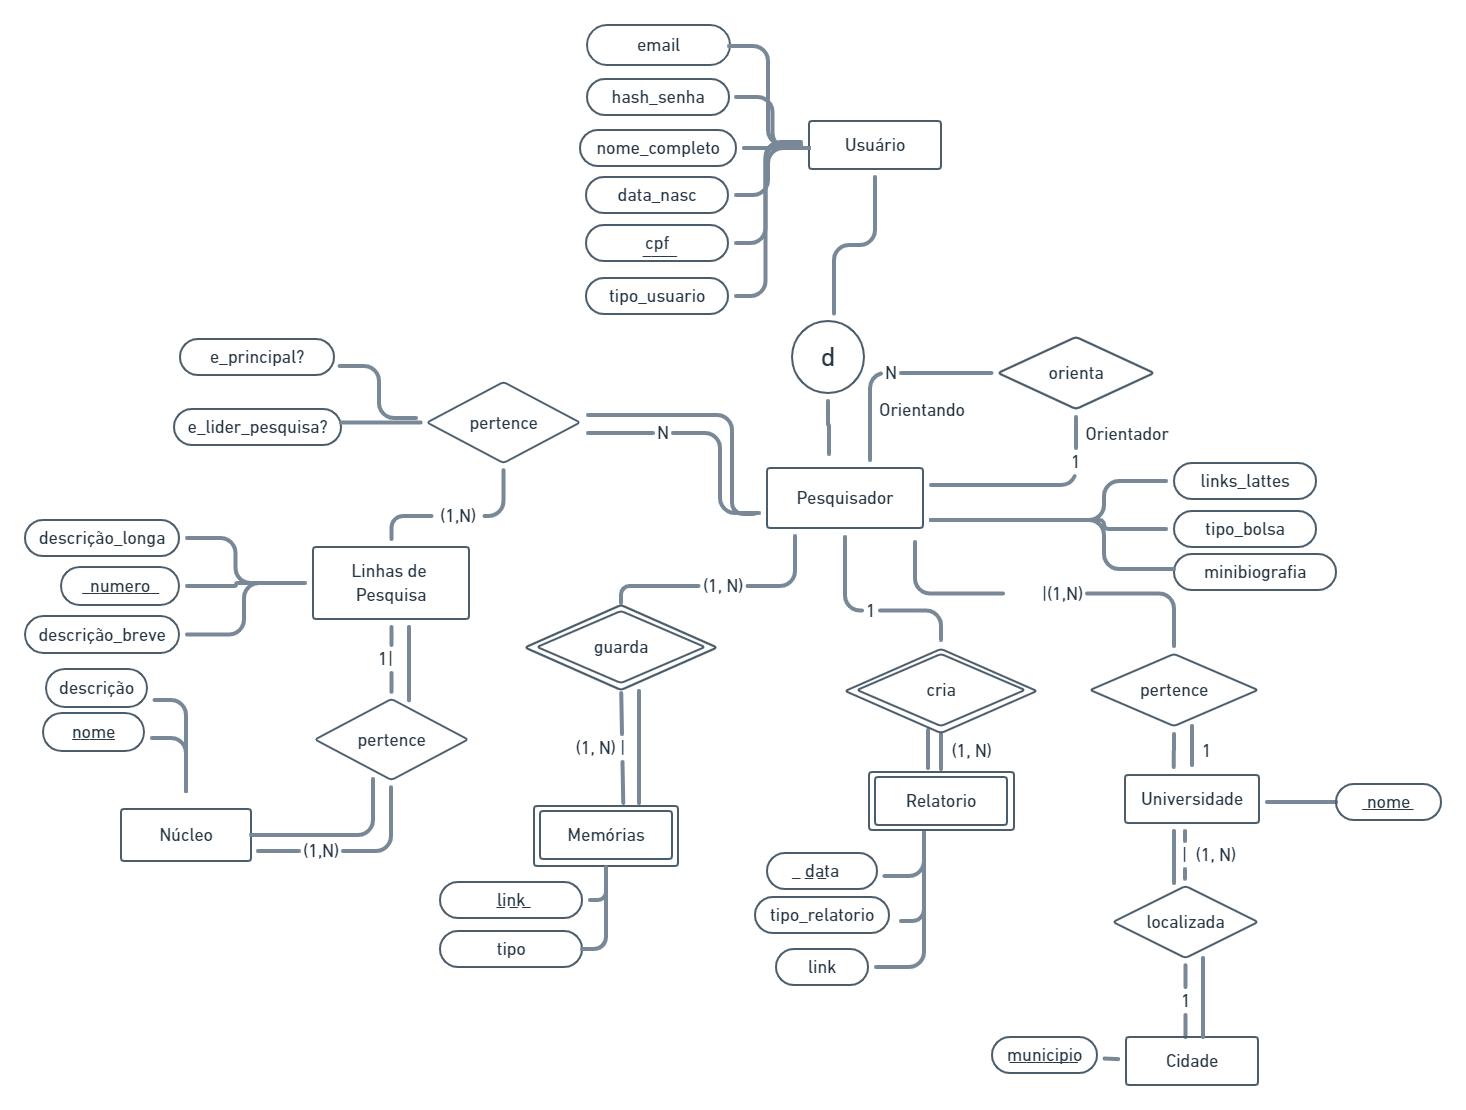
\includegraphics[width=17cm]{figuras/Diagrama2.png}
    \caption{Diagrama}
    \label{fig:logolatex}
\end{figure}
\clearpage



\section{Projeto Conceitual}

\begin{table}[h]
    \centering
    \vspace{0.5cm}
    \begin{tabular}{ |p{2,5cm}|p{3cm}|p{4cm}|p{5,3cm}|  }
        \hline
        Tipo-Entidade & Atributo         & Tipo            & Restrições                                                      \\ % Note a separação de col. e a quebra de linhas


        \hline
                      & papeis           & Identificador   & Gerado Automaticamente                                          \\
        Linhas        & Número           & Monovalorasdo   & Obrigatório                                                     \\
        de Pesquisa   & Descrição        & Monovalorado    & Opcional, <= 280 caracteres                                     \\

        \hline
        Núcleos       & Nome do Núcleo   & Chave candidata & Obrigatório                                                     \\
                      & Descrição Núcleo & Monovalorado    & Obrigatório, <= 400 caracteres                                  \\
        \hline
                      & Código Memórias  & Identificador   & Gerado Automaticamente                                          \\
        Memórias      & Links fotos      & Monovalorado    & Obrigatório                                                     \\
        \hline
                      & Cancelada?       & Monovalorado    & Opcional, padrão: false                                         \\
        Reuniões      & Data agendada    & Monovalorado    & Obrigatório                                                     \\
                      & Tipo             & Monovalorado    & Lideres\linebreak Núcleos\linebreak Geral\linebreak Excepcional \\

        \hline
    \end{tabular}
    \caption{Tipos de atributos por tipo-entidade do DER.}
\end{table}
\clearpage
\begin{table}[h]
    \centering
    \vspace{0.5cm}
    \begin{tabular}{ |p{2,5cm}|p{3cm}|p{4cm}|p{5,3cm}|  }

        \hline
        Tipo-Entidade & Atributo                      & Tipo              & Restrições                                             \\ % Note a separação de col. e a quebra de linhas

        \hline
        % para uma linha horizontal
                      & Cpf                           & Identificador     & Gerado Automaticamente                                 \\
                      & E-mail                        & Chave candidata   & Obrigatório, formato válido                            \\
        Usuários      & Senha                         & Monovalorado      & Obrigatório                                            \\
                      & Nome completo                 & Chave candidata   & Obrigatório                                            \\
                      & Hash Senha                    & Monovalorado      & Obrigatório                                            \\
                      & Tipo                          & Monovalorado      & Administrador\linebreak Pesquisador\linebreak Pescador \\
        \hline


                      & Link Lattes                   & Chave candidata   & Obrigatório                                            \\
                      & Tipo de bolsa                 & Monovalorado      & Obrigatório                                            \\
                      & Cidade                        & Monovalorado      & Obrigatório                                            \\
        Pesquisador   & Universidade                  & Monovalorado      & Obrigatório                                            \\
                      & Orientandos                   & Monovalorado      & Obrigatório                                            \\
                      & Minibiografia                 & Monovalorado      & Obrigatório, <= 280 caracteres                         \\                                     \\
                      & Código\linebreak LP principal & Chave estrangeira & Obrigatório                                            \\



        \hline



                      & Autor                        & Monovalorado      & Obrigatório                                            \\
        Relatório     &                   & Monovalorado      & Obrigatório                                            \\
                      & Tipo                   & Monovalorado      & Mensal\linebreak Trimestral\linebreak Anual\linebreak                                            \\
    \end{tabular}
    \caption{Tipos de atributos por tipo-entidade do DER.}
\end{table}

\clearpage

% ----------------------------------------------------------
% Referências bibliográficas
% ----------------------------------------------------------
\bibliography{referencias}        %use a bibtex bibliography file refs.bib


\begin{itemize}
    \item \href{https://github.com/cciuenf/pea_pescarte/blob/main/doc_projeto/documentos/fluxograma_modulos.pdf}{Fluxograma Módulos PEA Pescarte }

\end{itemize}

\end{document}

